%        File: report.tex
%     Created: Wed Sep 19 09:00 AM 2018 C
% Last Change: Wed Sep 19 09:00 AM 2018 C
%
\documentclass[letterpaper]{article}
\usepackage[top=1.0in,bottom=1.0in,left=1.0in,right=1.0in]{geometry}
\usepackage{verbatim}
\usepackage{amssymb}
\usepackage{graphicx}
\usepackage{longtable}
\usepackage{amsfonts}
\usepackage{amsmath}
\usepackage{hyperref}
\def\thesection       {\arabic{section}}
\def\thesubsection     {\thesection.\alph{subsection}}

\author{Your Name
        \\ \href{mailto:YOUREMAIL@illinois.edu}{\texttt{YOUREMAIL@illinois.edu}}
}

\title{Course Number\\
Assignment Title\\
Assignment Number}
\begin{document}
%\clearpage
\begin{titlepage}
\maketitle
\thispagestyle{empty}
\end{titlepage}

\section{Introduction}
Text should be clear and understandable in full sentences with no grammar errors. Equations should be edited with the equation editor and should include numbers where needed. This is handled automagically by \LaTeX. 

\begin{align}
E=mc^2\label{eq:relativity}
\end{align}
You can even reference equations like equation \ref{eq:relativity} easily.

\section{Analytical Solution}

More text follows. And maybe you need to reference a paper about depletion \cite{gauld_isotopic_2011}.

\section{Results}
All of the figures and such will need to be presented nicely as is Figure 
\ref{fig:alpha} below. Please note that you should reference all figures in the 
text.

\begin{figure}[htbp!]
        \begin{center}
                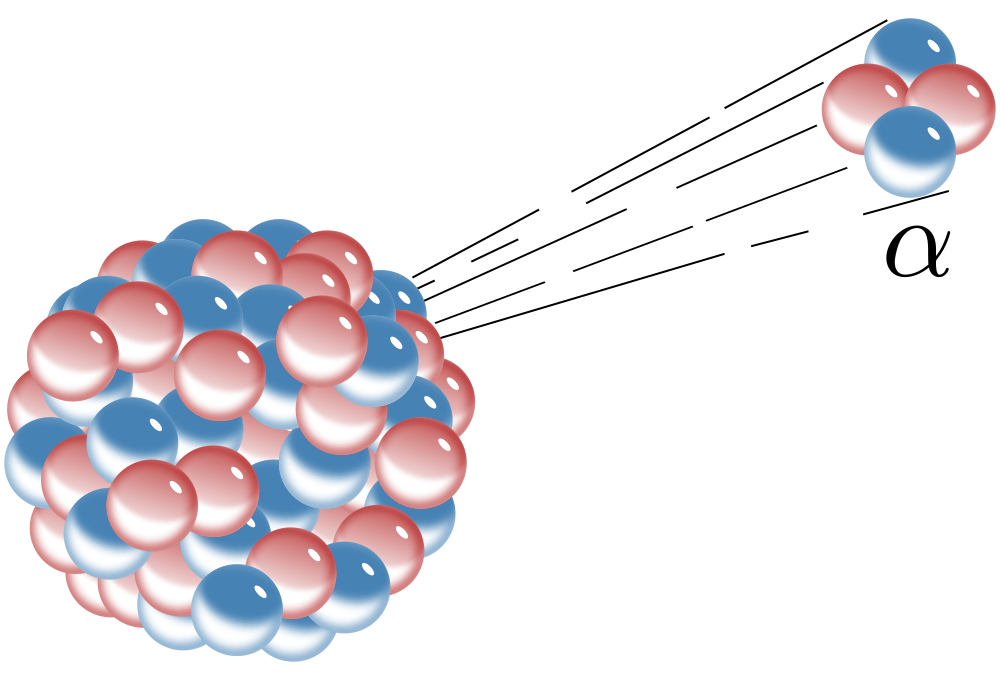
\includegraphics[width=0.3\textwidth]{./imgs/alpha_decay.png}
        \end{center}
        \caption{This image, of $\alpha$ emission from a large nucleus,  was 
        created by Inductiveload from Wikimedia Commons and is in the public 
        domain. Accordingly, I don't need to cite it, but I can attribute it anyway.}
        \label{fig:alpha}
\end{figure}


\pagebreak
\bibliographystyle{plain}
\bibliography{bibliography}
\end{document}


